\documentclass[14pt]{extbook}
\usepackage{multicol, enumerate, enumitem, hyperref, color, soul, setspace, parskip, fancyhdr} %General Packages
\usepackage{amssymb, amsthm, amsmath, latexsym, units, mathtools} %Math Packages
\everymath{\displaystyle} %All math in Display Style
% Packages with additional options
\usepackage[headsep=0.5cm,headheight=12pt, left=1 in,right= 1 in,top= 1 in,bottom= 1 in]{geometry}
\usepackage[usenames,dvipsnames]{xcolor}
\usepackage{dashrule}  % Package to use the command below to create lines between items
\newcommand{\litem}[1]{\item#1\hspace*{-1cm}\rule{\textwidth}{0.4pt}}
\pagestyle{fancy}
\lhead{Progress Quiz 7}
\chead{}
\rhead{Version B}
\lfoot{3510-5252}
\cfoot{}
\rfoot{Summer C 2021}
\begin{document}

\begin{enumerate}
\litem{
Choose the equation of the function graphed below.
\begin{center}
    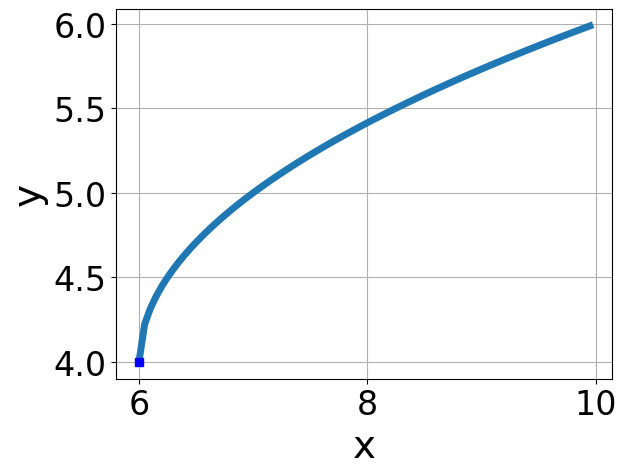
\includegraphics[width=0.5\textwidth]{../Figures/radicalGraphToEquationCopyB.png}
\end{center}
\begin{enumerate}[label=\Alph*.]
\item \( f(x) = \sqrt{x + 6} + 4 \)
\item \( f(x) = - \sqrt{x + 6} + 4 \)
\item \( f(x) = - \sqrt{x - 6} + 4 \)
\item \( f(x) = \sqrt{x - 6} + 4 \)
\item \( \text{None of the above} \)

\end{enumerate} }
\litem{
Choose the graph of the equation below.\[ f(x) = - \sqrt{x - 8} + 3 \]\begin{enumerate}[label=\Alph*.]
\begin{multicols}{2}\item 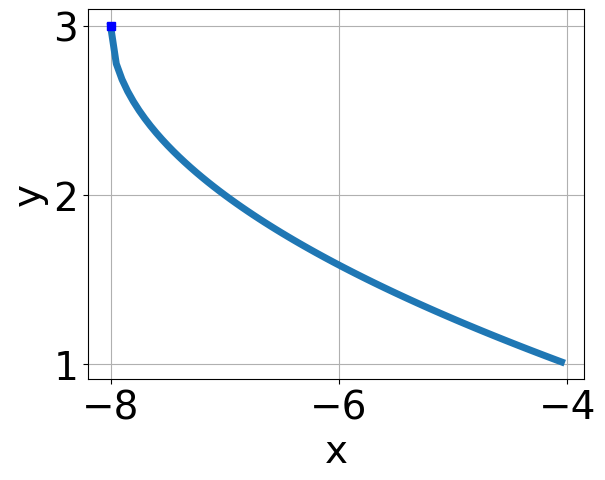
\includegraphics[width = 0.3\textwidth]{../Figures/radicalEquationToGraphAB.png}\item 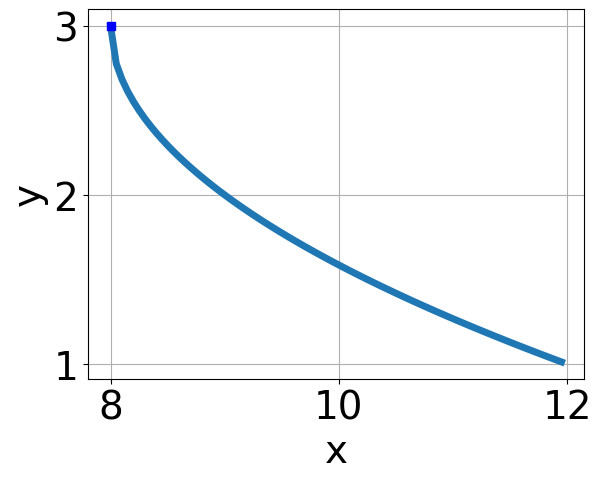
\includegraphics[width = 0.3\textwidth]{../Figures/radicalEquationToGraphBB.png}\item 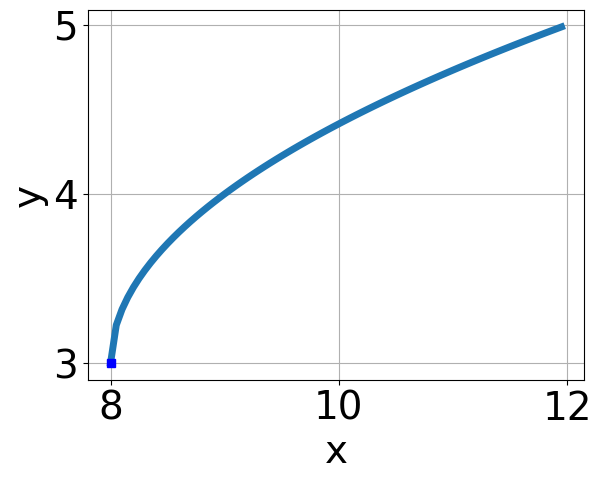
\includegraphics[width = 0.3\textwidth]{../Figures/radicalEquationToGraphCB.png}\item 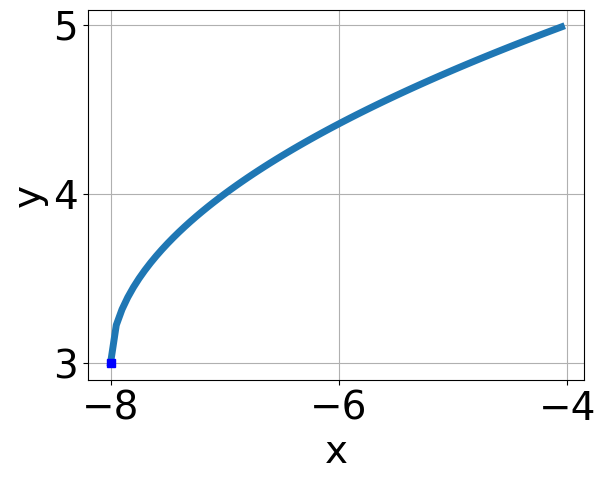
\includegraphics[width = 0.3\textwidth]{../Figures/radicalEquationToGraphDB.png}\end{multicols}\item None of the above.
\end{enumerate} }
\litem{
Solve the radical equation below. Then, choose the interval(s) that the solution(s) belongs to.\[ \sqrt{63 x^2 + 10} - \sqrt{59 x} = 0 \]\begin{enumerate}[label=\Alph*.]
\item \( x_1 \in [-0.44, 0.67] \text{ and } x_2 \in [0.6,2.1] \)
\item \( x_1 \in [-0.88, -0.67] \text{ and } x_2 \in [-0.6,-0.1] \)
\item \( x \in [0.27,1.08] \)
\item \( \text{All solutions lead to invalid or complex values in the equation.} \)
\item \( x \in [-0.44,0.67] \)

\end{enumerate} }
\litem{
Choose the equation of the function graphed below.
\begin{center}
    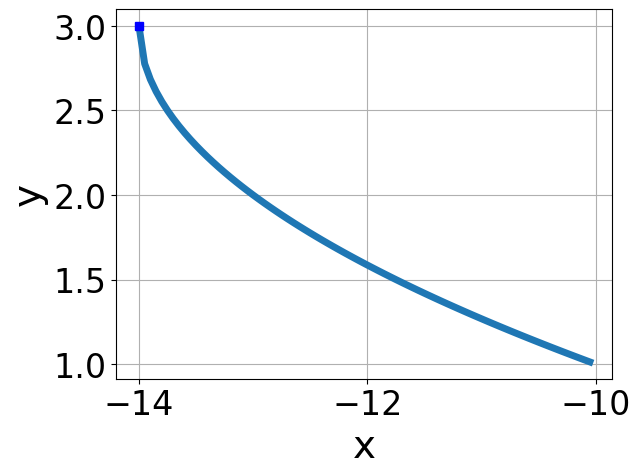
\includegraphics[width=0.5\textwidth]{../Figures/radicalGraphToEquationB.png}
\end{center}
\begin{enumerate}[label=\Alph*.]
\item \( f(x) = \sqrt{x + 14} + 3 \)
\item \( f(x) = - \sqrt{x - 14} + 3 \)
\item \( f(x) = \sqrt{x - 14} + 3 \)
\item \( f(x) = - \sqrt{x + 14} + 3 \)
\item \( \text{None of the above} \)

\end{enumerate} }
\litem{
Solve the radical equation below. Then, choose the interval(s) that the solution(s) belongs to.\[ \sqrt{-12 x^2 + 30} - \sqrt{-2 x} = 0 \]\begin{enumerate}[label=\Alph*.]
\item \( x_1 \in [1.3, 1.55] \text{ and } x_2 \in [-3.33,2.67] \)
\item \( x_1 \in [-1.64, -1.4] \text{ and } x_2 \in [-3.33,2.67] \)
\item \( \text{All solutions lead to invalid or complex values in the equation.} \)
\item \( x \in [-1.64,-1.4] \)
\item \( x \in [1.6,1.77] \)

\end{enumerate} }
\litem{
Solve the radical equation below. Then, choose the interval(s) that the solution(s) belongs to.\[ \sqrt{-4 x + 8} - \sqrt{-9 x - 6} = 0 \]\begin{enumerate}[label=\Alph*.]
\item \( x_1 \in [-1.21, -0.61] \text{ and } x_2 \in [-2,7] \)
\item \( x_1 \in [-3.15, -2.55] \text{ and } x_2 \in [-2,7] \)
\item \( x \in [-3.15,-2.55] \)
\item \( x \in [-0.45,0.32] \)
\item \( \text{All solutions lead to invalid or complex values in the equation.} \)

\end{enumerate} }
\litem{
What is the domain of the function below?\[ f(x) = \sqrt[5]{-6 x + 4} \]\begin{enumerate}[label=\Alph*.]
\item \( \text{The domain is } (-\infty, a], \text{   where } a \in [-5.2, 1.4] \)
\item \( \text{The domain is } (-\infty, a], \text{   where } a \in [1.2, 1.9] \)
\item \( (-\infty, \infty) \)
\item \( \text{The domain is } [a, \infty), \text{   where } a \in [1.32, 1.96] \)
\item \( \text{The domain is } [a, \infty), \text{   where } a \in [-0.15, 1.37] \)

\end{enumerate} }
\litem{
Choose the graph of the equation below.\[ f(x) = - \sqrt{x + 6} - 5 \]\begin{enumerate}[label=\Alph*.]
\begin{multicols}{2}\item 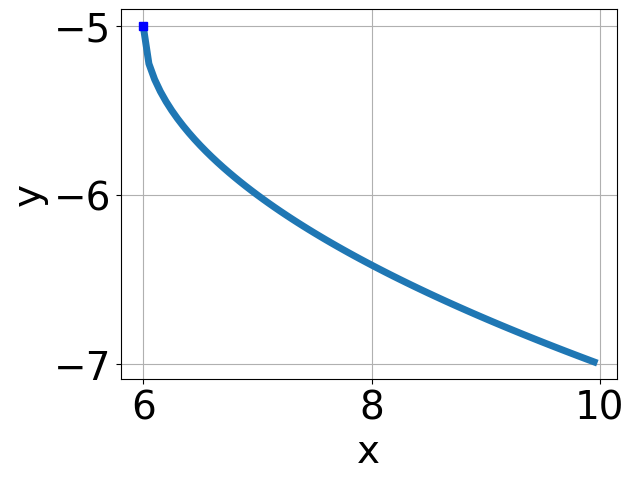
\includegraphics[width = 0.3\textwidth]{../Figures/radicalEquationToGraphCopyAB.png}\item 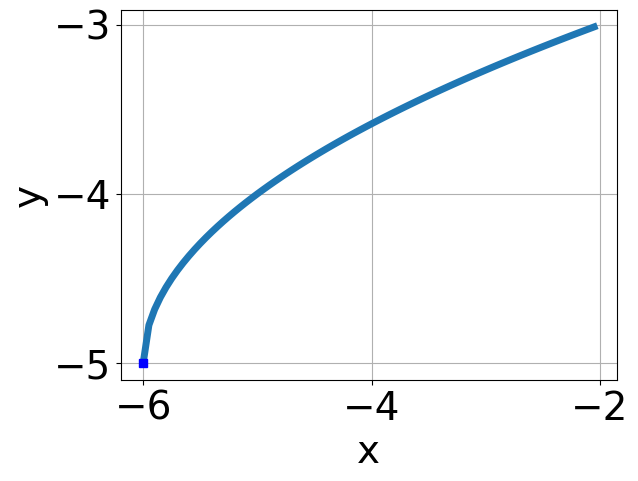
\includegraphics[width = 0.3\textwidth]{../Figures/radicalEquationToGraphCopyBB.png}\item 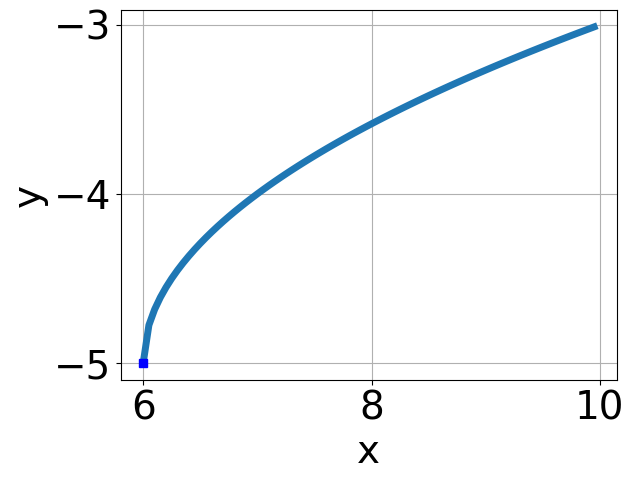
\includegraphics[width = 0.3\textwidth]{../Figures/radicalEquationToGraphCopyCB.png}\item 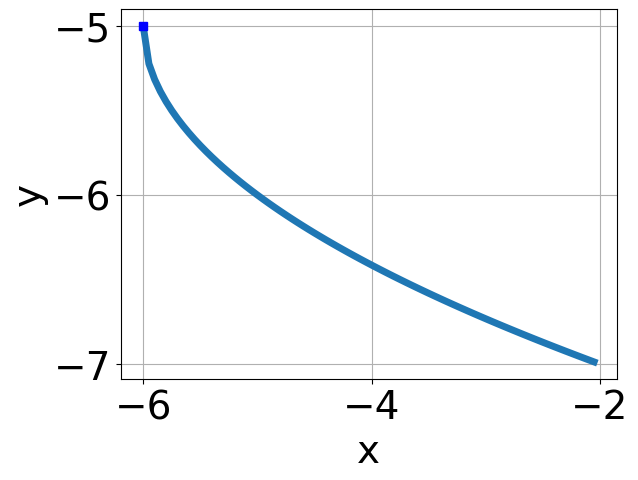
\includegraphics[width = 0.3\textwidth]{../Figures/radicalEquationToGraphCopyDB.png}\end{multicols}\item None of the above.
\end{enumerate} }
\litem{
What is the domain of the function below?\[ f(x) = \sqrt[6]{3 x + 6} \]\begin{enumerate}[label=\Alph*.]
\item \( [a, \infty), \text{where } a \in [-0.6, 0.2] \)
\item \( (-\infty, a], \text{where } a \in [-2.3, -1.5] \)
\item \( (-\infty, a], \text{where } a \in [-1.8, 0.5] \)
\item \( (-\infty, \infty) \)
\item \( [a, \infty), \text{ where } a \in [-2.8, -0.7] \)

\end{enumerate} }
\litem{
Solve the radical equation below. Then, choose the interval(s) that the solution(s) belongs to.\[ \sqrt{7 x + 6} - \sqrt{9 x - 9} = 0 \]\begin{enumerate}[label=\Alph*.]
\item \( x \in [7.22,8.19] \)
\item \( x_1 \in [-1.3, 0.85] \text{ and } x_2 \in [-1,4] \)
\item \( x_1 \in [-1.3, 0.85] \text{ and } x_2 \in [5.5,11.5] \)
\item \( \text{All solutions lead to invalid or complex values in the equation.} \)
\item \( x \in [-3.06,-0.9] \)

\end{enumerate} }
\end{enumerate}

\end{document}